% Options for packages loaded elsewhere
\PassOptionsToPackage{unicode}{hyperref}
\PassOptionsToPackage{hyphens}{url}
%
\documentclass[
  8pt,
  ignorenonframetext,
]{beamer}
\usepackage{pgfpages}
\setbeamertemplate{caption}[numbered]
\setbeamertemplate{caption label separator}{: }
\setbeamercolor{caption name}{fg=normal text.fg}
\beamertemplatenavigationsymbolsempty
% Prevent slide breaks in the middle of a paragraph
\widowpenalties 1 10000
\raggedbottom
\setbeamertemplate{part page}{
  \centering
  \begin{beamercolorbox}[sep=16pt,center]{part title}
    \usebeamerfont{part title}\insertpart\par
  \end{beamercolorbox}
}
\setbeamertemplate{section page}{
  \centering
  \begin{beamercolorbox}[sep=12pt,center]{part title}
    \usebeamerfont{section title}\insertsection\par
  \end{beamercolorbox}
}
\setbeamertemplate{subsection page}{
  \centering
  \begin{beamercolorbox}[sep=8pt,center]{part title}
    \usebeamerfont{subsection title}\insertsubsection\par
  \end{beamercolorbox}
}
\AtBeginPart{
  \frame{\partpage}
}
\AtBeginSection{
  \ifbibliography
  \else
    \frame{\sectionpage}
  \fi
}
\AtBeginSubsection{
  \frame{\subsectionpage}
}
\usepackage{amsmath,amssymb}
\usepackage{lmodern}
\usepackage{iftex}
\ifPDFTeX
  \usepackage[T1]{fontenc}
  \usepackage[utf8]{inputenc}
  \usepackage{textcomp} % provide euro and other symbols
\else % if luatex or xetex
  \usepackage{unicode-math}
  \defaultfontfeatures{Scale=MatchLowercase}
  \defaultfontfeatures[\rmfamily]{Ligatures=TeX,Scale=1}
\fi
% Use upquote if available, for straight quotes in verbatim environments
\IfFileExists{upquote.sty}{\usepackage{upquote}}{}
\IfFileExists{microtype.sty}{% use microtype if available
  \usepackage[]{microtype}
  \UseMicrotypeSet[protrusion]{basicmath} % disable protrusion for tt fonts
}{}
\makeatletter
\@ifundefined{KOMAClassName}{% if non-KOMA class
  \IfFileExists{parskip.sty}{%
    \usepackage{parskip}
  }{% else
    \setlength{\parindent}{0pt}
    \setlength{\parskip}{6pt plus 2pt minus 1pt}}
}{% if KOMA class
  \KOMAoptions{parskip=half}}
\makeatother
\usepackage{xcolor}
\newif\ifbibliography
\setlength{\emergencystretch}{3em} % prevent overfull lines
\providecommand{\tightlist}{%
  \setlength{\itemsep}{0pt}\setlength{\parskip}{0pt}}
\setcounter{secnumdepth}{-\maxdimen} % remove section numbering
% type setting
% ------------------------------------------------------------------------------
\usepackage[german]{babel}     

% fonts
% ------------------------------------------------------------------------------
\usefonttheme{professionalfonts}

% slide title and horizontal line
% ------------------------------------------------------------------------------
\setbeamertemplate{frametitle}{%
    \vskip-30pt \color{black}\large%
    \begin{minipage}[b][23pt]{120mm}%
    \flushleft\insertframetitle%
    \end{minipage}%
}

\setbeamertemplate{headline}										
{
\vskip10pt\hfill\hspace{3.5mm} 										 
\vskip15pt\color{black}\rule{\textwidth}{0.4pt} 					 
}

% slide number
% ---------------------------------------------------------------
\setbeamertemplate{navigation symbols}{}
\setbeamertemplate{footline}
{
\vskip5pt
\vskip2pt
\makebox[123mm]{\hspace{7.5mm}
\hfill Psychologische Forschungsmethoden $\vert$ 
\copyright $ $ 2022 Dirk Ostwald CC BY-NC-SA 4.0 $\vert$ 
Folie \insertframenumber}
\vskip4pt
}

% block color scheme
% ------------------------------------------------------------------------------
% colors
\definecolor{white}{RGB}{255,255,255}
\definecolor{grey}{RGB}{235,235,235}
\definecolor{lightgrey}{RGB}{245,245,245}
\definecolor{LightBlue}{RGB}{220,220,255}
\definecolor{darkblue}{RGB}{51, 51, 153}

% definitions and theorems
\setbeamercolor{block title}{fg = black, bg = grey}
\setbeamercolor{block body}{fg = black, bg = lightgrey}

% general line spacing 
% ------------------------------------------------------------------------------
\linespread{1.3}

% local line spacing
% ------------------------------------------------------------------------------
\usepackage{setspace}

% colors
% -----------------------------------------------------------------------------
\usepackage{color}

% justified text
% ------------------------------------------------------------------------------
\usepackage{ragged2e}
\usepackage{etoolbox}
\apptocmd{\frame}{}{\justifying}{}

% bullet point lists
% -----------------------------------------------------------------------------
\setbeamertemplate{itemize item}[circle]
\setbeamertemplate{itemize subitem}[circle]
\setbeamertemplate{itemize subsubitem}[circle]
\setbeamercolor{itemize item}{fg = black}
\setbeamercolor{itemize subitem}{fg = black}
\setbeamercolor{itemize subsubitem}{fg = black}
\setbeamercolor{enumerate item}{fg = black}
\setbeamercolor{enumerate subitem}{fg = black}
\setbeamercolor{enumerate subsubitem}{fg = black}
\setbeamerfont{itemize/enumerate body}{}
\setbeamerfont{itemize/enumerate subbody}{size = \normalsize}
\setbeamerfont{itemize/enumerate subsubbody}{size = \normalsize}

% color links
% ------------------------------------------------------------------------------
\usepackage{hyperref}
\definecolor{urls}{RGB}{204,0,0}
\hypersetup{colorlinks, citecolor = darkblue, urlcolor = urls}


% additional math commands
% ------------------------------------------------------------------------------
\usepackage{bm}                                         % bold math symbols
\newcommand{\niton}{\not\owns}

% text highlighting
% ------------------------------------------------------------------------------
\usepackage{soul}
\makeatletter
\let\HL\hl
\renewcommand\hl{%
  \let\set@color\beamerorig@set@color
  \let\reset@color\beamerorig@reset@color
  \HL}
\makeatother

% equation highlighting
% -----------------------------------------------------------------------------
\newcommand{\highlight}[2][yellow]{\mathchoice%
  {\colorbox{#1}{$\displaystyle#2$}}%
  {\colorbox{#1}{$\textstyle#2$}}%
  {\colorbox{#1}{$\scriptstyle#2$}}%
  {\colorbox{#1}{$\scriptscriptstyle#2$}}}%

% additional mathematical operators
% ------------------------------------------------------------------------------
\DeclareMathOperator*{\argmax}{arg\,max}
\DeclareMathOperator*{\argmin}{arg\,min}

\ifLuaTeX
  \usepackage{selnolig}  % disable illegal ligatures
\fi
\IfFileExists{bookmark.sty}{\usepackage{bookmark}}{\usepackage{hyperref}}
\IfFileExists{xurl.sty}{\usepackage{xurl}}{} % add URL line breaks if available
\urlstyle{same} % disable monospaced font for URLs
\hypersetup{
  hidelinks,
  pdfcreator={LaTeX via pandoc}}

\author{}
\date{\vspace{-2.5em}}

\begin{document}

\begin{frame}[plain]{}
\protect\hypertarget{section}{}
\center

\begin{center}
\includegraphics[width=0.2\linewidth]{0_Abbildungen/pfm_0_otto} \end{center}

\vspace{2mm}

\Large

Psychologische Forschungsmethoden \vspace{6mm}

\normalsize

BSc Philosophie-Neurowissenschaften-Kognition WiSe 22/23

BSc Psychologie WiSe 22/23

\large
\vspace{6mm}

Prof.~Dr.~Dirk Ostwald
\end{frame}

\begin{frame}[plain]{}
\protect\hypertarget{section-1}{}
\Huge
\vfill
\center

\textcolor{red}{Aufnahme läuft!} \vfill
\end{frame}

\begin{frame}[plain]{}
\protect\hypertarget{section-2}{}
\vfill
\center
\huge

\textcolor{black}{(0) Formalia} \vfill
\end{frame}

\begin{frame}{Formalia}
\protect\hypertarget{formalia}{}
\vfill
\begin{large}
Prof. Dr. Dirk Ostwald (dirk.ostwald@ovgu.de)
\end{large}
\vspace{.7cm}

\begin{minipage}{.3\linewidth}
\begin{center}
\includegraphics[scale=.6]{0_Abbildungen/pfm_0_dirk.pdf}
\end{center}
\end{minipage}
\begin{minipage}{.7\linewidth}
\begin{small}
\renewcommand{\arraystretch}{1.3}
\begin{tabular}{ll}
Seit 2021   & W2 Professur Methodenlehre I                    \\
2014 - 2020 & W1 Professur Freie Universität Berlin       \\
2010 - 2014 & Postdoc BCCN \& MPIB Berlin                       \\
2007 - 2010 & PhD Psychologie Birmingham                        \\
2004 - 2006 & MSc Neurowissenschaften Tübingen              \\
2005 - 2012 & BSc Mathematik Hagen                                \\
2000 - 2003 & BSc Medizin Hamburg                                   \\
\end{tabular}
\end{small}
\end{minipage}
\vspace{.7cm}

\begin{large}
\begin{tabular}{ll}
Forschung   & Komputationale Kognitive Neurowissenschaften  \\
Lehre         & Datenwissenschaft
\end{tabular}
\end{large}
\vfill
\end{frame}

\begin{frame}{}
\protect\hypertarget{section-3}{}
\large

\href{https://www.ipsy.ovgu.de/methodenlehre_I-path-980,1404.html}{\textcolor{darkblue}{Homepage}}
\vspace{2mm}

\begin{center}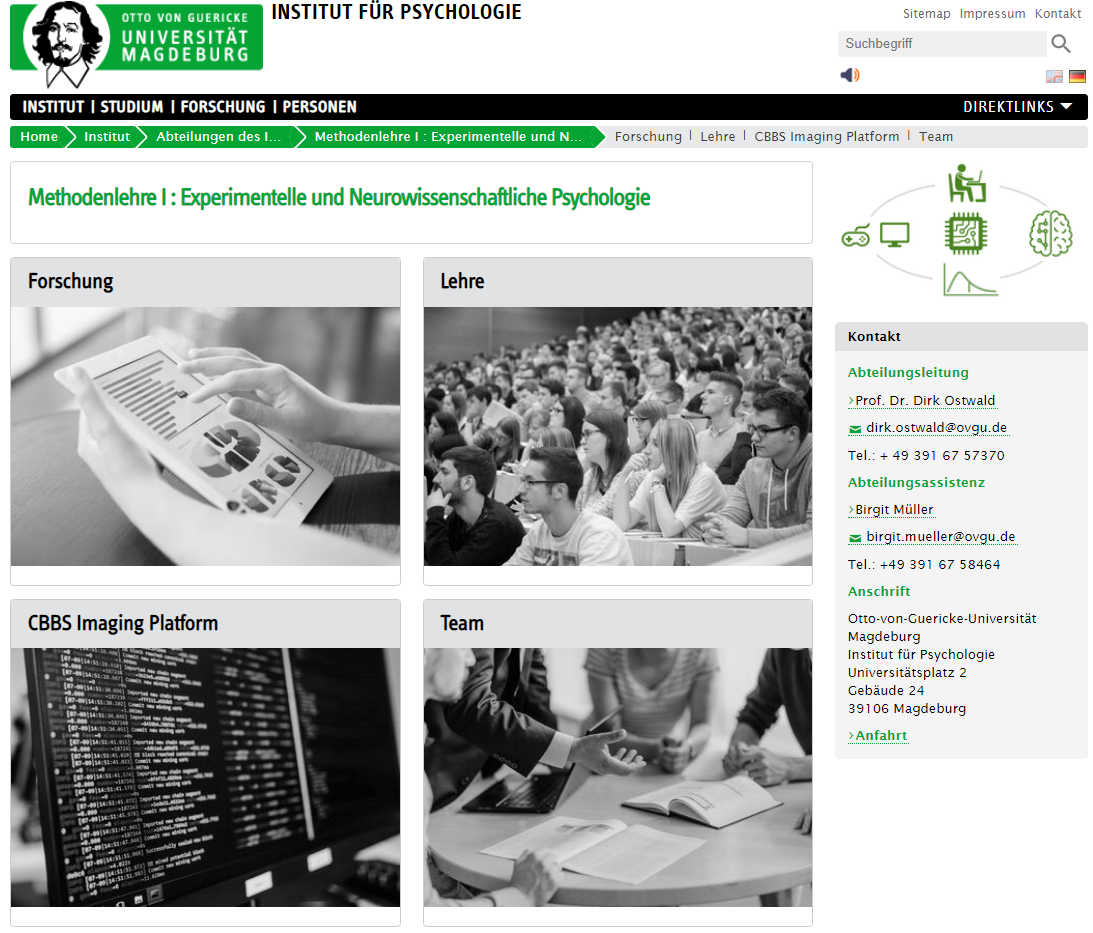
\includegraphics[width=0.7\linewidth]{0_Abbildungen/pfm_0_homepage} \end{center}
\end{frame}

\begin{frame}{Formalia}
\protect\hypertarget{formalia-1}{}
\large
\setstretch{2}

\textcolor{darkblue}{Terminierung der Vorlesung}

\normalsize

\begin{itemize}
\tightlist
\item
  Mögliche Live-Alternativen: Do 9 - 11 Uhr, Do 11 - 13 Uhr, Fr 14 - 16
  Uhr
\item
  Vorlesung online verfügbar
\item
  Verlegung abhängig von Raumverfügbarkeit
\end{itemize}

\textcolor{darkblue}{Bitte organisieren Sie sich und weisen Sie eine Mehrheitsentscheidung digital nach!}
\end{frame}

\begin{frame}{Formalia}
\protect\hypertarget{formalia-2}{}
\vspace{2mm}

\textcolor{darkblue}{Datenanalytisches Curriculum im 1. Studienjahr BSc Psychologie}
\small \setstretch{1.6}

\underline{Erstes Semester}

\begin{itemize}
\tightlist
\item
  Vorkurs Fit für Psychologie

  \begin{itemize}
  \tightlist
  \item
    \small Mathematische und informatische Grundlagen
  \end{itemize}
\item
  \textcolor{darkblue}{A2. Einführung in die Forschungsmethoden der Psychologie}

  \begin{itemize}
  \tightlist
  \item
    \small \textcolor{darkblue}{Das Große Ganze zur wissenschaftlichen Psychologie und Messtheorie}
  \end{itemize}
\item
  B1. Deskriptivstatistik

  \begin{itemize}
  \tightlist
  \item
    \small Wahrscheinlichkeitstheorie und Frequentistische Inferenz
  \end{itemize}
\item
  C1. Einführung in empirisch-wissenschaftliches Arbeiten

  \begin{itemize}
  \tightlist
  \item
    \small Programmierung und Deskriptive Statistik
  \end{itemize}
\end{itemize}

\vspace{-1mm}

\underline{Zweites Semester}

\begin{itemize}
\tightlist
\item
  B2. Inferenzstatistik

  \begin{itemize}
  \tightlist
  \item
    \small Das Allgemeine Lineare Modell
  \end{itemize}
\item
  C2. Einführung in empirisch-wissenschaftliches Arbeiten

  \begin{itemize}
  \tightlist
  \item
    \small Dokumentation und Präsentation
  \end{itemize}
\end{itemize}
\end{frame}

\begin{frame}{Formalia}
\protect\hypertarget{formalia-3}{}
\textcolor{darkblue}{Modul A2. Einführung in die Forschungsmethoden der Psychologie}
\setstretch{2}

\begin{itemize}
\tightlist
\item
  Donnerstag 7.00 - 9.00 Uhr in Raum G40B-238 (?)
\item
  Kursmaterialien (Folien, Videos, RMarkdown Code) auf der
  \href{https://bit.ly/3T6BcoQ}{\textcolor{darkblue}{Kurswebseite}}
\item
  Code auf
  \href{https://github.com/dirk-ostwald/psychologische-forschungsmethoden-23}{\textcolor{darkblue}{Github}}
\item
  Ankündigungen über die
  \href{https://elearning.ovgu.de/course/view.php?id=13818}{\textcolor{darkblue}{Moodleseite}}
\item
  \href{https://bit.ly/3SNh3nR}{\textcolor{darkblue}{Link zum Kurs Mathematische Grundlagen}}
\item
  \href{https://bit.ly/3MmsfFK}{\textcolor{darkblue}{Link zur vorherigen Iteration des Kurses}}
\end{itemize}

\flushright

\(\Rightarrow\) Grundlegende Überarbeitung im WiSe 22/23!
\end{frame}

\begin{frame}[t]{Formalia}
\protect\hypertarget{formalia-4}{}
\vspace{1mm}

\textcolor{darkblue}{Vorläufige Vorlesungsübersicht}

\small
\center
\footnotesize
\renewcommand{\arraystretch}{1.1}
\begin{tabular}{lll}
Datum        & Einheit                       & Thema                                            \\\hline
13.10.2022   & Formalia                      & (0) Formalia                             \\
13.10.2022   & Psychologische Wissenschaft   & (1) Wissenschaft                         \\
20.10.2022   & Psychologische Wissenschaft   & (2) Psychologische Forschung             \\
27.10.2022   & Psychologische Wissenschaft   & (3) Psychologische Daten                 \\
03.11.2022   & Messtheorie                   & (4) Grundlagen                           \\
10.11.2022   & Messtheorie                   & (5) Nominales Messen                     \\
17.11.2022   & Messtheorie                   & (6) Ordinales Messen                     \\
24.11.2022   & Messtheorie                   & (7) Extensives Messen                    \\
01.12.2022   & Messtheorie                   & (8) Differenzmessungen                   \\
08.12.2022   & Messtheorie                   & (9) Praktische Messtheorie               \\
15.12.2022   & Stichprobentheorie            & (10) Grundlagen                          \\
05.01.2023   & Stichprobentheorie            & (11) Stratifizierte Stichproben          \\
12.01.2023   & Stichprobentheorie            & (12) Cluster Stichproben                   \\
19.01.2023   & Quasiexperimentelle Methoden  & (13) Grundlagen                          \\
26.01.2023   & Quasiexperimentelle Methoden  & (14) Propensity Scores                   \\\hline
Feb  2023    & Klausurtermin                 &                                          \\
Juli 2023    & Klausurwiederholungstermin    &
\end{tabular}
\end{frame}

\begin{frame}{Formalia}
\protect\hypertarget{formalia-5}{}
\textcolor{darkblue}{Modul A2. Einführung in die Forschungsmethoden der Psychologie}
\setstretch{2}

\begin{itemize}
\tightlist
\item
  Vorlesungsfolien inklusive Selbstkontrollfragen sind klausurrelevant
\item
  Selbstkontrollfragen fokussieren den Kursinhalt
\item
  Selbstkontrollfragen sind Grundlage für Prüfungsfragen
\item
  Benotete Multiple Choice Klausur (20 Fragen) Ende WiSe 2022/23
\item
  Gemeinsame Klausur mit Modul A1. Einführung in die Psychologie und
  ihre Geschichte
\item
  Klausurwiederholungstermin am Ende SoSe 2023
\item
  Klausurtermin und Klausurort gemäß Prüfungsplan des
  \href{https://www.fnw.ovgu.de/Studium/Pr\%C3\%BCfungsamt.html}{FNW
  Prüfungsamtes}
\end{itemize}
\end{frame}

\begin{frame}{Formalia}
\protect\hypertarget{formalia-6}{}
\Huge
\vfill
\center

Q \& A \vfill
\end{frame}

\end{document}
